\section{Overlays}

\subsection{Usages}

\begin{frame}{\textbackslash pause}
	The command \textbackslash pause makes the text following it to be shown only from the next slide on, which is a command using \textbackslash onslide internally.

	An example:
	\begin{itemize}
		\pause
		\item One
		\pause
		\item Two
		\pause
		\item Three
	\end{itemize}
\end{frame}

\begin{frame}{\textbackslash uncover, \textbackslash visible \& \textbackslash only}
	\begin{description}
		\item[\textbackslash uncover] The text occupies space and is still typeset, but it is not shown or only shown as if transparent
		\item[\textbackslash visible] It is almost the same as \textbackslash uncover, except that if the text is not shown, it is never shown transparently, but rather it is not shown at all
		\item[\textbackslash only] The text is inserted only into the specified slides and for other slides, it is thrown away and occupies no space
	\end{description}
\end{frame}

\subsection{Examples}

\begin{frame}{Examples of \textbackslash uncover, \textbackslash visible \& \textbackslash only}
	A labelling is a set of local labelling functions.

	\begin{itemize}
		\uncover<1->{\item The vertex-labelled graph \(G\)}
		\uncover<2->{\item The local labelling function \alert{\(f_{v_3}\)}, for \(f_{v_3}(v_2) = 2\) and \(f_{v_3}(v_4) = 1\)}
		\uncover<3->{\item The labelling \(\textbf{f} = \{\, f_{v_1}, f_{v_2}, \alert{f_{v_3}}, f_{v_3}, f_{v_4}, f_{v_5} \,\}\)}
	\end{itemize}

	\begin{figure}[ht]
		\centering
		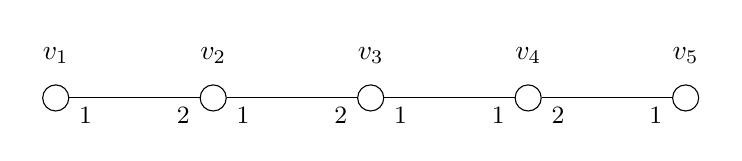
\begin{tikzpicture}
	\visible<1->
	{
		\begin{scope}[every node/.style = {circle, draw}]
			\node (v1) [label = above:$v_1$] at (180: 2 * 2) {};
			\node (v2) [label = above:$v_2$] at (180: 2) {};
			\node (v3) [label = above:$v_3$] at (0, 0) {};
			\node (v4) [label = above:$v_4$] at (0: 2) {};
			\node (v5) [label = above:$v_5$] at (0: 2 * 2) {};
		\end{scope}

		\path (v1) edge (v2);
		\path (v2) edge (v3);
		\path (v3) edge (v4);
		\path (v4) edge (v5);
	}

	\visible<2->
	{
		\path (v3) edge node [very near start, below] {\small \alert{2}} (v2);
		\path (v3) edge node [very near start, below] {\small \alert{1}} (v4);
	}

	\visible<3->
	{
		\path (v1) edge node [very near start, below] {\small 1} node [very near end, below] {\small 2} (v2);
		\path (v2) edge node [very near start, below] {\small 1} (v3);
		\path (v3) edge node [very near end, below] {\small 1} (v4);
		\path (v4) edge node [very near start, below] {\small 2} node [very near end, below] {\small 1} (v5);
	}
\end{tikzpicture}

	\end{figure}
\end{frame}

\begin{frame}{Examples of \textbackslash uncover, \textbackslash visible \& \textbackslash only (Cont.)}
	\begin{figure}[ht]
		\centering
		\only<1-3>
		{
			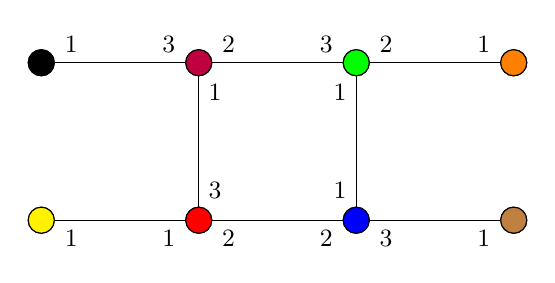
\begin{tikzpicture}
	\visible<1-2>
	{
		\begin{scope}[every node/.style = {circle, draw}]
			\node (v1) at (0, 0) {};
			\node (v2) at (2, 0) {};
			\node (v3) at (0, -2) {};
			\node (v4) at (2, -2) {};
			\node (v5) at (-2, 0) {};
			\node (v6) at (2 * 2, 0) {};
			\node (v7) at (-2, -2) {};
			\node (v8) at (2 * 2, -2) {};
		\end{scope}

		\path (v1) edge (v2);
		\path (v1) edge (v3);
		\path (v1) edge (v5);
		\path (v2) edge (v4);
		\path (v2) edge (v6);
		\path (v3) edge (v4);
		\path (v3) edge (v7);
		\path (v4) edge (v8);
	}

	\visible<2-3>
	{
		\path (v1) edge node [very near start, above] {\small 2} node [very near end, above] {\small 3} (v2);
		\path (v1) edge node [very near start, right] {\small 1} node [very near end, right] {\small 3} (v3);
		\path (v1) edge node [very near start, above] {\small 3} node [very near end, above] {\small 1} (v5);
		\path (v2) edge node [very near start, left] {\small 1} node [very near end, left] {\small 1} (v4);
		\path (v2) edge node [very near start, above] {\small 2} node [very near end, above] {\small 1} (v6);
		\path (v3) edge node [very near start, below] {\small 2} node [very near end, below] {\small 2} (v4);
		\path (v3) edge node [very near start, below] {\small 1} node [very near end, below] {\small 1} (v7);
		\path (v4) edge node [very near start, below] {\small 3} node [very near end, below] {\small 1} (v8);
	}

	\visible<3>
	{
		\begin{scope}[every node/.style = {circle, draw}]
			\node (v1) [fill = purple] at (0, 0) {};
			\node (v2) [fill = green] at (2, 0) {};
			\node (v3) [fill = red] at (0, -2) {};
			\node (v4) [fill = blue] at (2, -2) {};
			\node (v5) [fill = black] at (-2, 0) {};
			\node (v6) [fill = orange] at (2 * 2, 0) {};
			\node (v7) [fill = yellow] at (-2, -2) {};
			\node (v8) [fill = brown] at (2 * 2, -2) {};
		\end{scope}
	}
\end{tikzpicture}

			\uncover<2-3>{\caption{\(s_{\textbf{f}} = 1\)}}
		}
		\only<4-6>
		{
			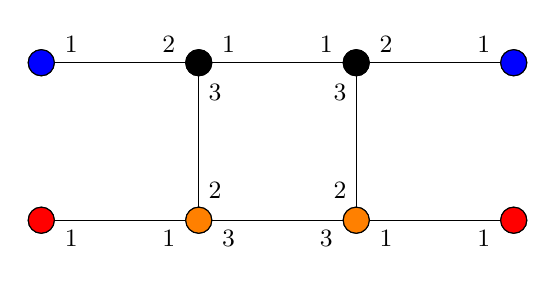
\begin{tikzpicture}
	\visible<4-5>
	{
		\begin{scope}[every node/.style = {circle, draw}]
			\node (v1) at (0, 0) {};
			\node (v2) at (2, 0) {};
			\node (v3) at (0, -2) {};
			\node (v4) at (2, -2) {};
			\node (v5) at (-2, 0) {};
			\node (v6) at (2 * 2, 0) {};
			\node (v7) at (-2, -2) {};
			\node (v8) at (2 * 2, -2) {};
		\end{scope}

		\path (v1) edge (v2);
		\path (v1) edge (v3);
		\path (v1) edge (v5);
		\path (v2) edge (v4);
		\path (v2) edge (v6);
		\path (v3) edge (v4);
		\path (v3) edge (v7);
		\path (v4) edge (v8);
	}

	\visible<5-6>
	{
		\path (v1) edge node [very near start, above] {\small 1} node [very near end, above] {\small 1} (v2);
		\path (v1) edge node [very near start, right] {\small 3} node [very near end, right] {\small 2} (v3);
		\path (v1) edge node [very near start, above] {\small 2} node [very near end, above] {\small 1} (v5);
		\path (v2) edge node [very near start, left] {\small 3} node [very near end, left] {\small 2} (v4);
		\path (v2) edge node [very near start, above] {\small 2} node [very near end, above] {\small 1} (v6);
		\path (v3) edge node [very near start, below] {\small 3} node [very near end, below] {\small 3} (v4);
		\path (v3) edge node [very near start, below] {\small 1} node [very near end, below] {\small 1} (v7);
		\path (v4) edge node [very near start, below] {\small 1} node [very near end, below] {\small 1} (v8);
	}

	\visible<6>
	{
		\begin{scope}[every node/.style = {circle, draw}]
			\node (v1) [fill = black] at (0, 0) {};
			\node (v2) [fill = black] at (2, 0) {};
			\node (v3) [fill = orange] at (0, -2) {};
			\node (v4) [fill = orange] at (2, -2) {};
			\node (v5) [fill = blue] at (-2, 0) {};
			\node (v6) [fill = blue] at (2 * 2, 0) {};
			\node (v7) [fill = red] at (-2, -2) {};
			\node (v8) [fill = red] at (2 * 2, -2) {};
		\end{scope}
	}
\end{tikzpicture}

			\uncover<5-6>{\caption{\(s_{\textbf{f}} = 2\)}}
		}
	\end{figure}
\end{frame}